\documentclass{article}

\usepackage[utf8]{inputenc}
\usepackage{graphicx}
\usepackage{url}
\usepackage{color}
\usepackage{titlesec}
\usepackage{amsmath}
\usepackage{physics}
\usepackage{amsfonts}
\usepackage{subcaption}
\usepackage{booktabs}
\graphicspath{{../figures/}}

\title{Declarative proto-paper for supersat project}
\author{K. Latimer}
\date{Nov 17, 2020}

\begin{document}

\maketitle

In order to determine experimental supersaturation within a reasonable margin of error, we must use the quasi-steady-state (QSS) supersaturation formula [cite]. Based on our analysis of the WRF data, this approximation is only valid within certain limits, namely:
\begin{itemize}
	\item T \textgreater  273K (we're not including ice in the theory; note that Fan et al do evaluate SS wrt water above the freezing line though)
	\item w \textgreater  2 m/s (reasonably strong updrafts)
	\item cloud LWC \textgreater  1e-4 g/g (in the convection core)
	\item including rain droplets and ventillation corrections
\end{itemize}

Figure \ref{wrfvsqss} shows a scatterplot with the agreement between the actual and QSS-derived SS values in the WRF simulation, for points satisfying the above criteria.

\clearpage
\newpage

\begin{figure}[ht]
	\centering
	\begin{subfigure}{0.7\textwidth}
		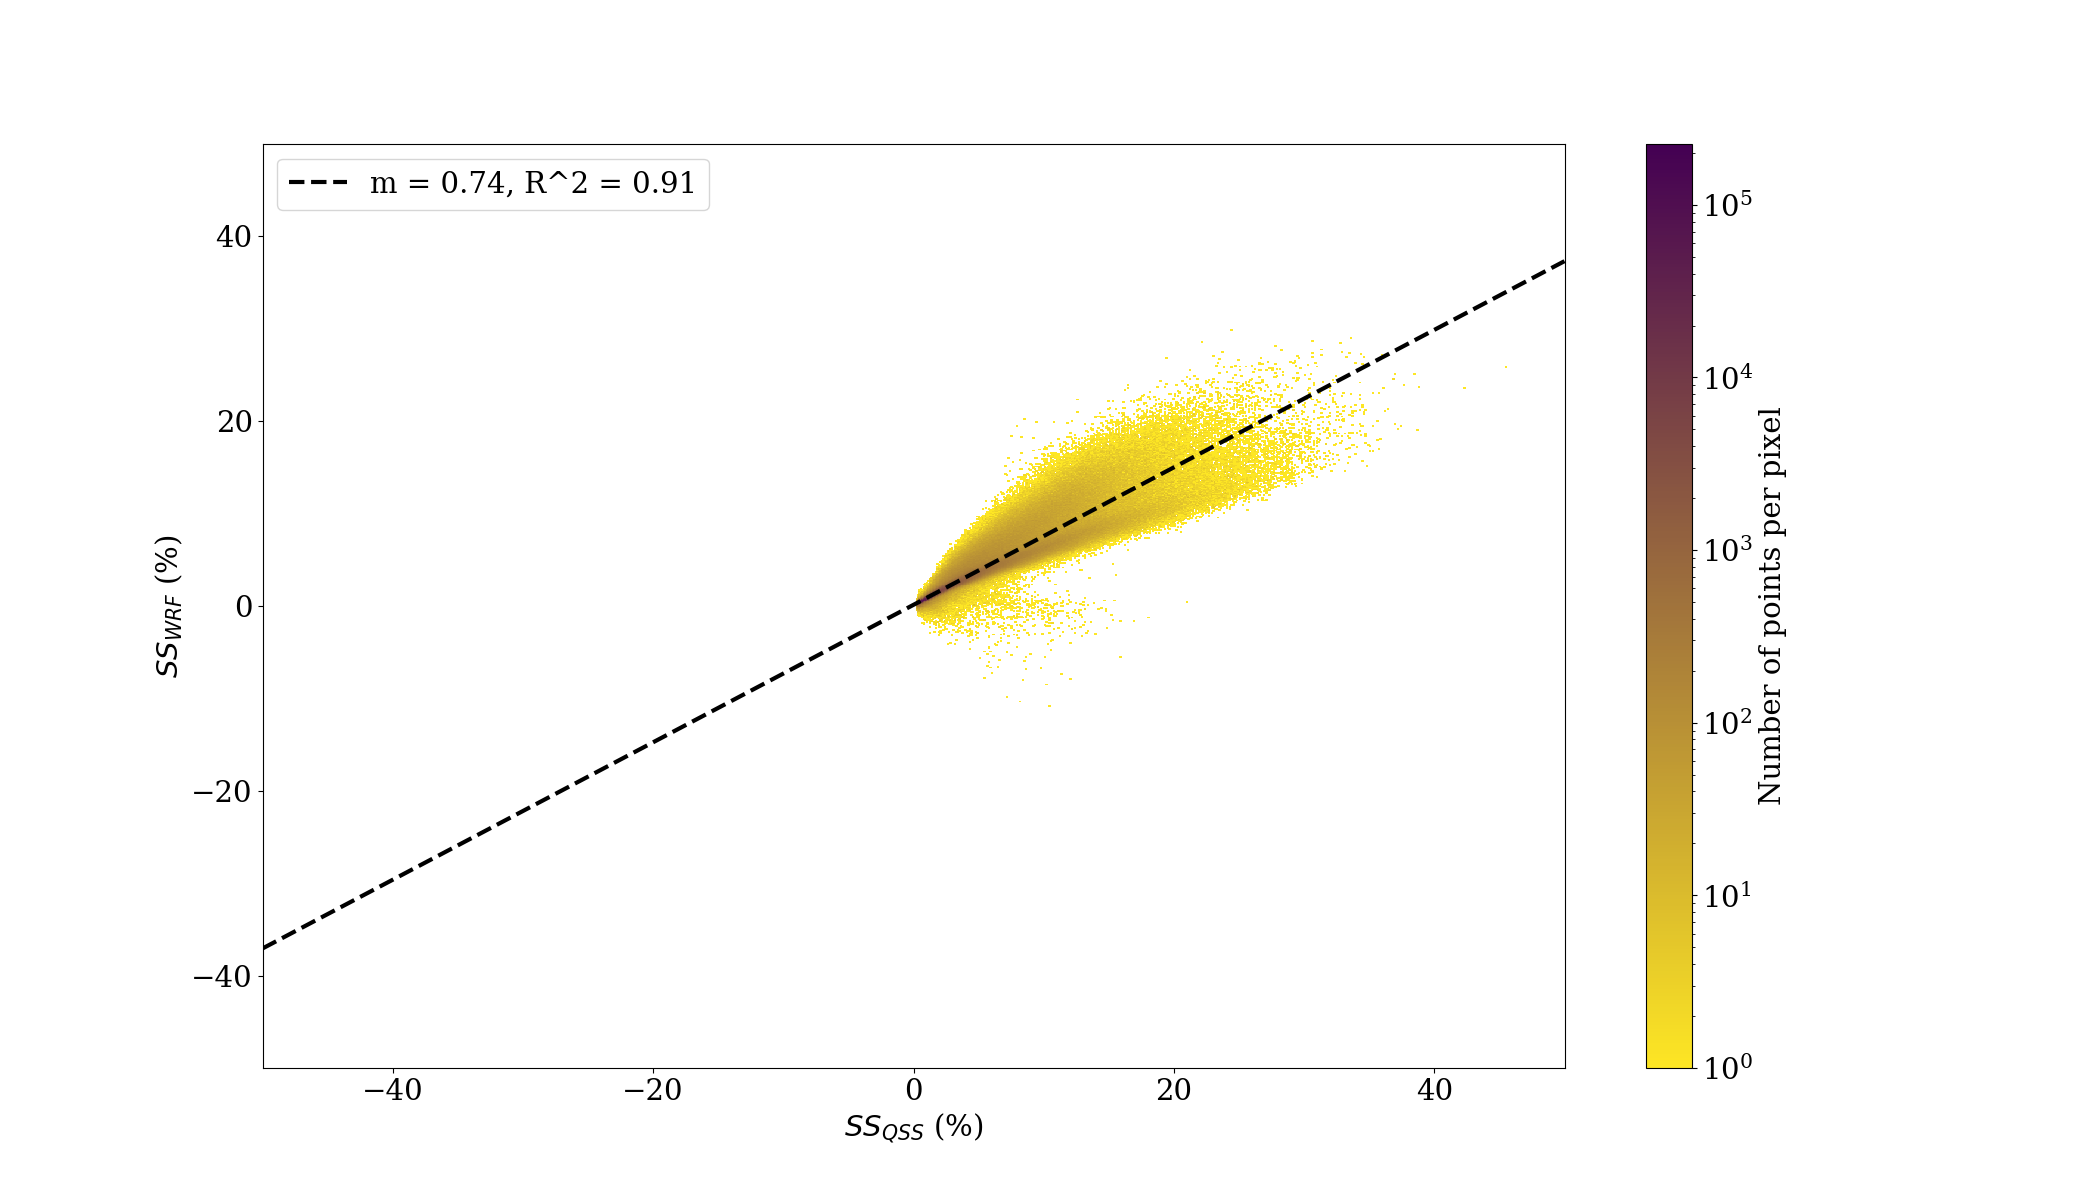
\includegraphics[width=\textwidth]{revmywrf/v12_heatmap_ss_qss_vs_ss_wrf_Unpolluted_figure_4.png}
		\caption{Unpolluted case.}
		\label{wrfvsqssunpoll}
	\end{subfigure}
	\begin{subfigure}{0.7\textwidth}
		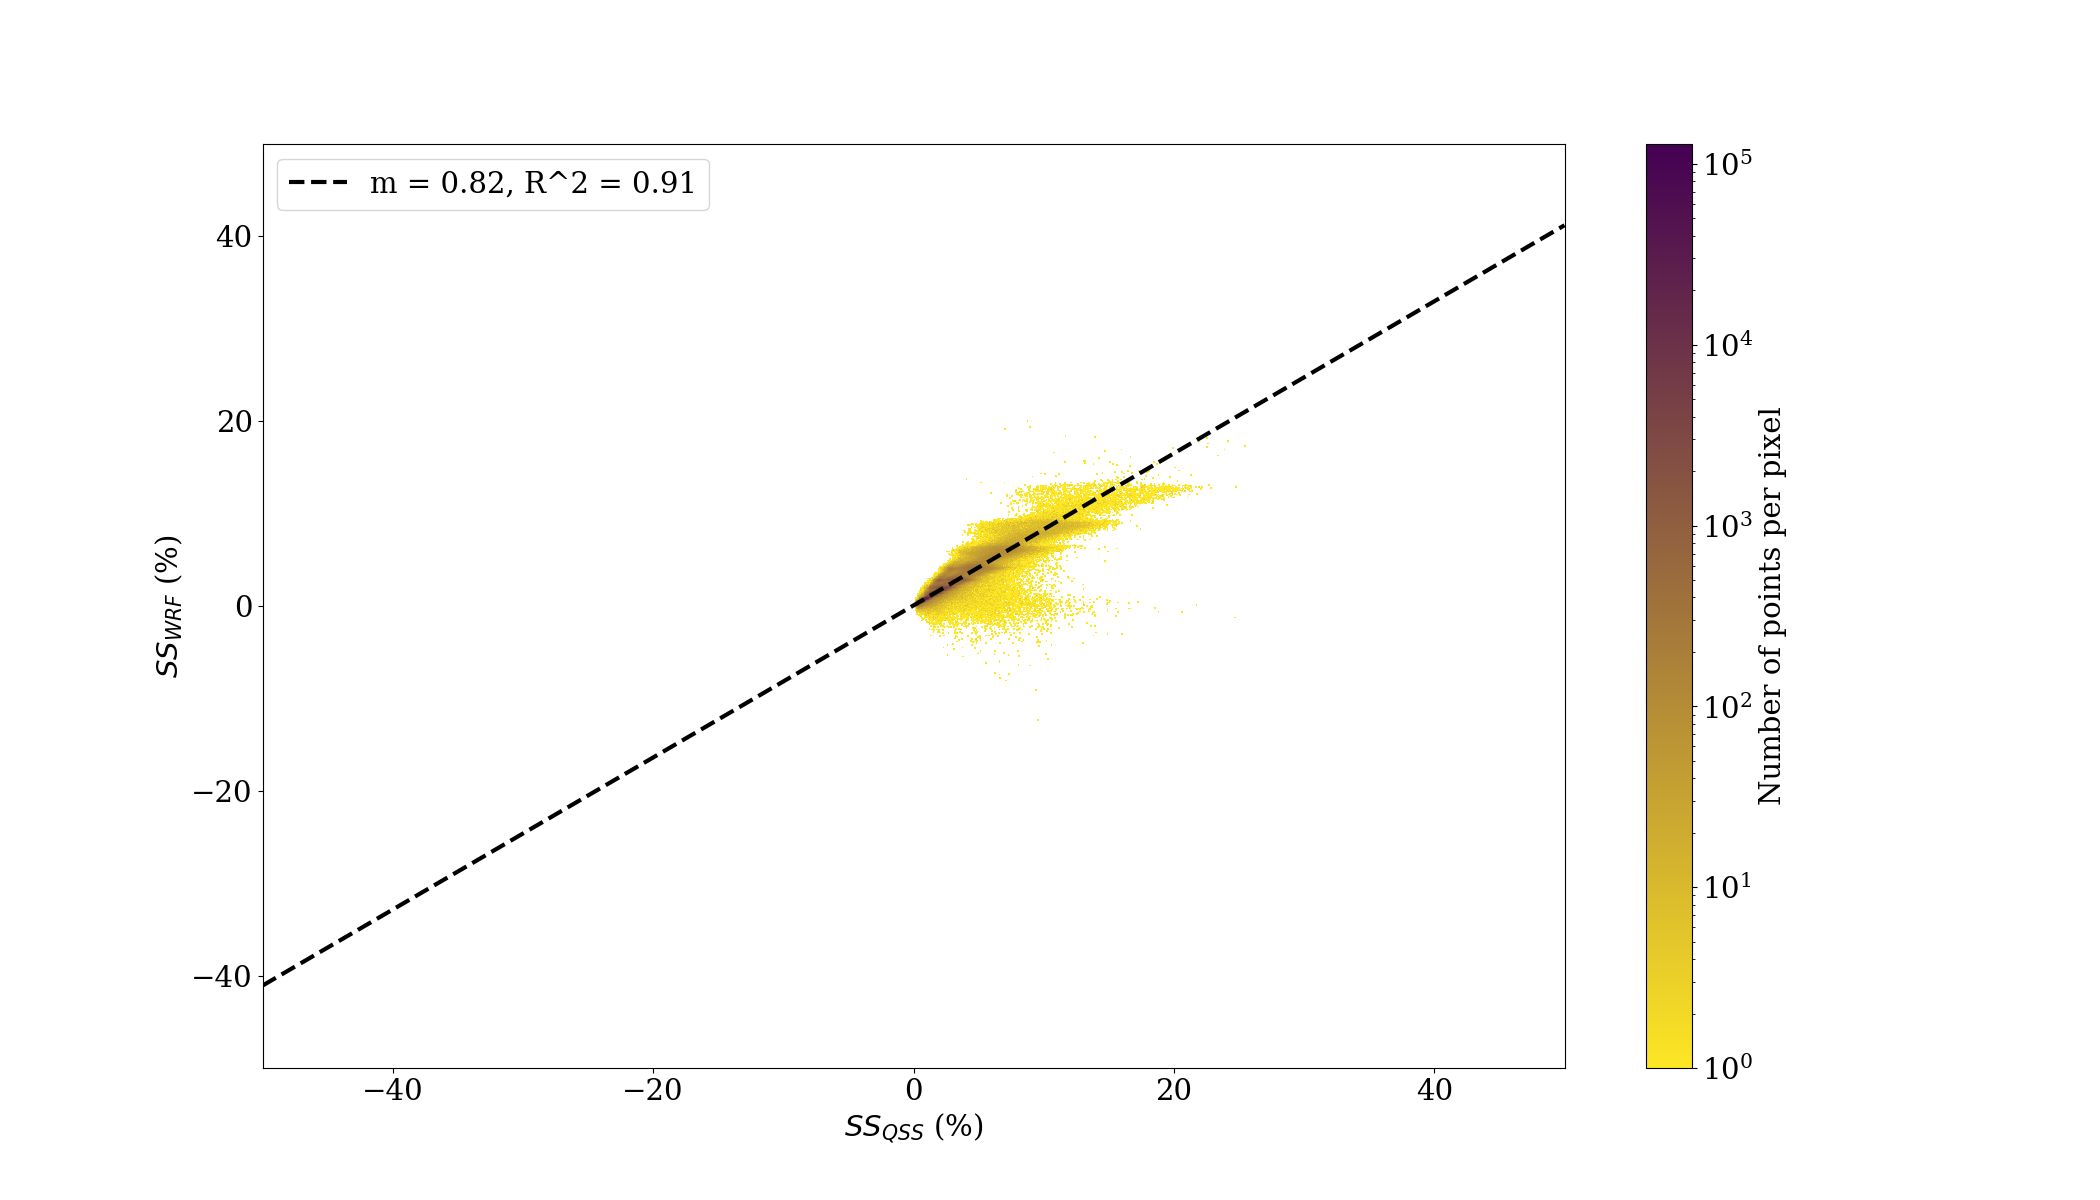
\includegraphics[width=\textwidth]{revmywrf/v12_heatmap_ss_qss_vs_ss_wrf_Polluted_figure_4.png}
		\caption{Polluted case.}
		\label{wrfvsqsspoll}
	\end{subfigure}
	\caption{Actual ($SS_{WRF}$) vs predicted ($SS_{QSS}$) supersaturation. Color indicates density of data points; note the scale is logarithmic.}
	\label{wrfvsqss}
\end{figure}

In Fan 2018, they claim that the so-called warm phase invigoration mechanism (WPIM) is driven by the presence of ultra-fine aerosol particles with sub-50nm diameters (UAP50) on the order of ~1000/ccm in the boundary layer (BL) where cloud droplets are nucleated. Crucial to this argument is the claim that, without such particles present, the troposphere supports very high supersaturations. In particular, this paper reports average supersaturations in the upper tenth percentile of updrafts in convective cells as high as $\approx$ 4 and 15\%, in the warm cloud and deep cloud phases \footnote{``Warm cloud" phase: ``30-min duration after the warm rain starts and the rain rate exceeds 0.5 mm/hour"; ``Deep cloud" phase: ``30-min duration with 15 min before and after the strongest convection."}, respectively, from WRF simulations of the pristine, pre-industrial Amazon rainforest. By contrast, the highest simulated supersaturations under typical modern-day pollution levels as observed in simulations were $\approx$ 1 and 6\%, respectively. 

In order to get a feel for how O(10\%) supersaturation would affect the energetics of a rising parcel of air relative to one with O(1\%) supersaturation, we estimate the difference in convective available potential energy (CAPE) between the two over the course of ascent. Assuming no heat of condensation is lost to the environment we have:
\begin{equation}
\label{energyconsv}
C_{ap}dT + L_vdq_v = 0,
\end{equation}
where $q_v$ is the water vapor mass fraction of the parcel ($q_v=m_v/m_{tot}$), also expressed in terms of the the relative humidity ($RH$) and saturation water vapor mass fraction ($q_v^*$) as:
\begin{equation}
\label{qveqn}
q_v = RHq_v^*
\end{equation}
The Clausius-Clayperon equation is:
\begin{equation}
\label{clauclay}
dq_v^* \approx \frac{q_v^*L_v}{R_vT^2}dT
\end{equation}
(The approximation is valid given that $\frac{L_v}{R_vT} \gg 1$.) Taking the differential of Equation \ref{qveqn} and rearranging terms in Equations \ref{energyconsv}, \ref{qveqn}, and \ref{clauclay} yields:
\begin{equation}
dT = \frac{-L_vq_v^*}{C_{pa} + q_v\frac{L_v^2}{R_vT^2}}dRH
\end{equation}
We suppose for the sake of this order-of-magnitude estimate that the difference in buoyancy between the two parcels is constant over a length scale of the troposphere's scale height (Is this a correct statement of the reasoning?? I am not sure if I understand why that is valid). Therefore the difference in CAPE is:
\begin{align}
dCAPE &\approx H \frac{dT}{T}\nonumber\\
&=H\frac{-L_vq_v^*}{T(C_{pa} + q_v\frac{L_v^2}{R_vT^2})}dRH\nonumber\\
&\approx 100 J/kg
\end{align}
(Converting directly to $\Delta KE$ this would translate to $ \Delta v\approx 15m/s$. I understand that total CAPE is not converted entirely to kinetic energy but given that we are comparing two parcels of the same mass ascending to the same height in the same environment, I'm not sure what else the difference in CAPE would translate to besides a difference in KE between the two? See annotated sketch in Figure \ref{capesketch}.)

\begin{figure}[ht]
    \centering
    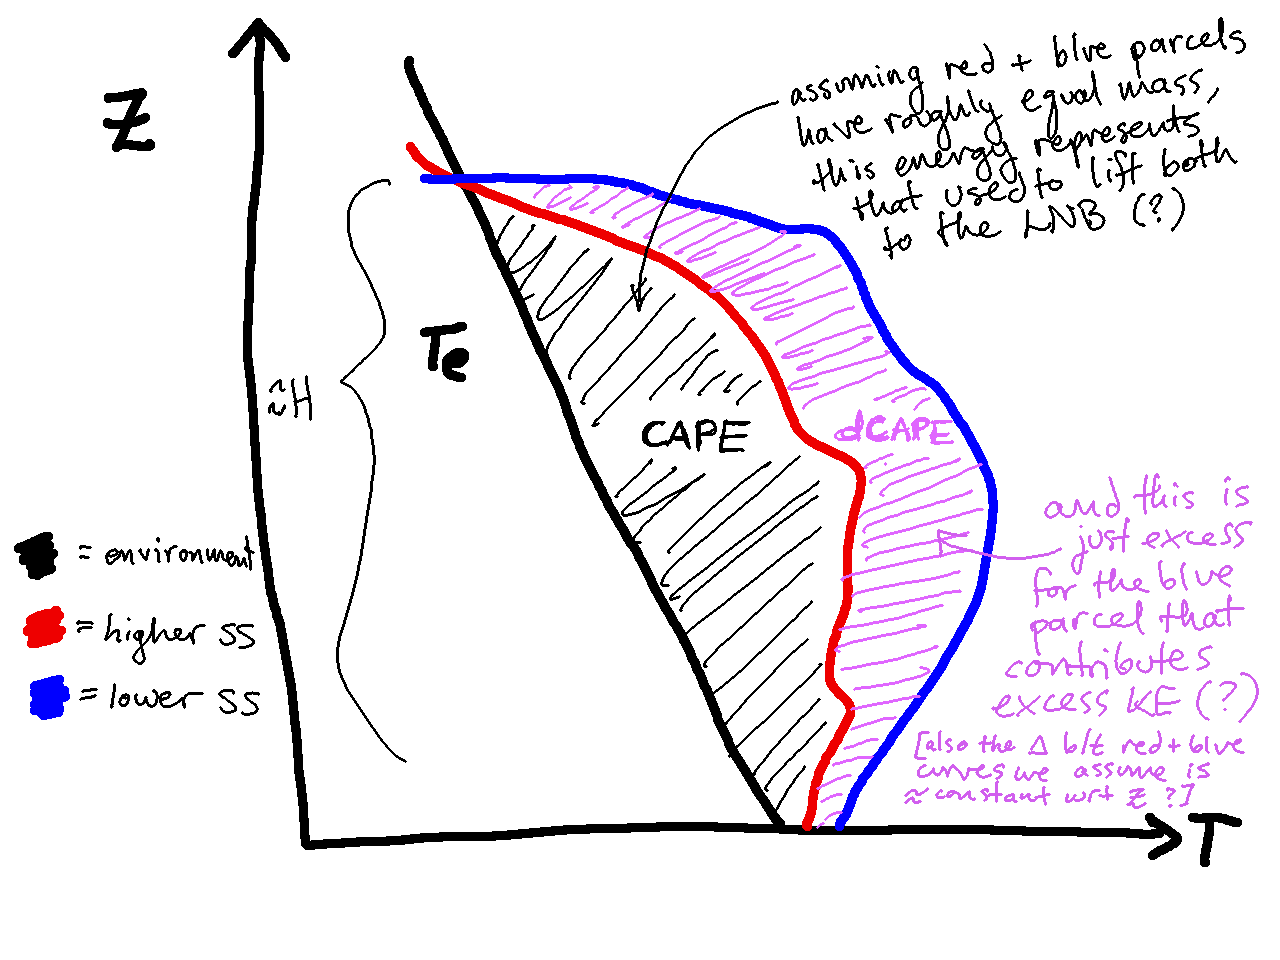
\includegraphics[width=12cm]{capesketch.png}
    \caption{Me trying to understand the meaning of the calculation above. Everything is extremely schematic.}
    \label{capesketch}
\end{figure}

We now seek to determine whether such high values actually occur in nature. First we look at data from the ACRIDICON-CHUVA mission (part of the HALO campaign) in the Amazon forest in Brazil. Aerosol concentrations in the BL (ie from ground-based measurements) both upwind and downwind of anthropogenic pollution sources on select flight dates are shown in Figures \ref{attoasd} and \ref{goaasd}, respectively.

\clearpage
\newpage

\begin{figure}[ht]
    \centering
    \includegraphics[width=9cm]{atto/atto_psd_figure.png}
    \caption{[DON'T HAVE DATA YET] Aerosol particle size distribution for a representative date; ground-based measurement coinciding with ACRIDICON-CHUVA flight dates, compared to initial distribution in boundary layer for WRF simulation. From ATTO site, upwind of Manaus metropolitan area.}
    \label{attoasd}
\end{figure}
\begin{figure}[ht]
    \centering
    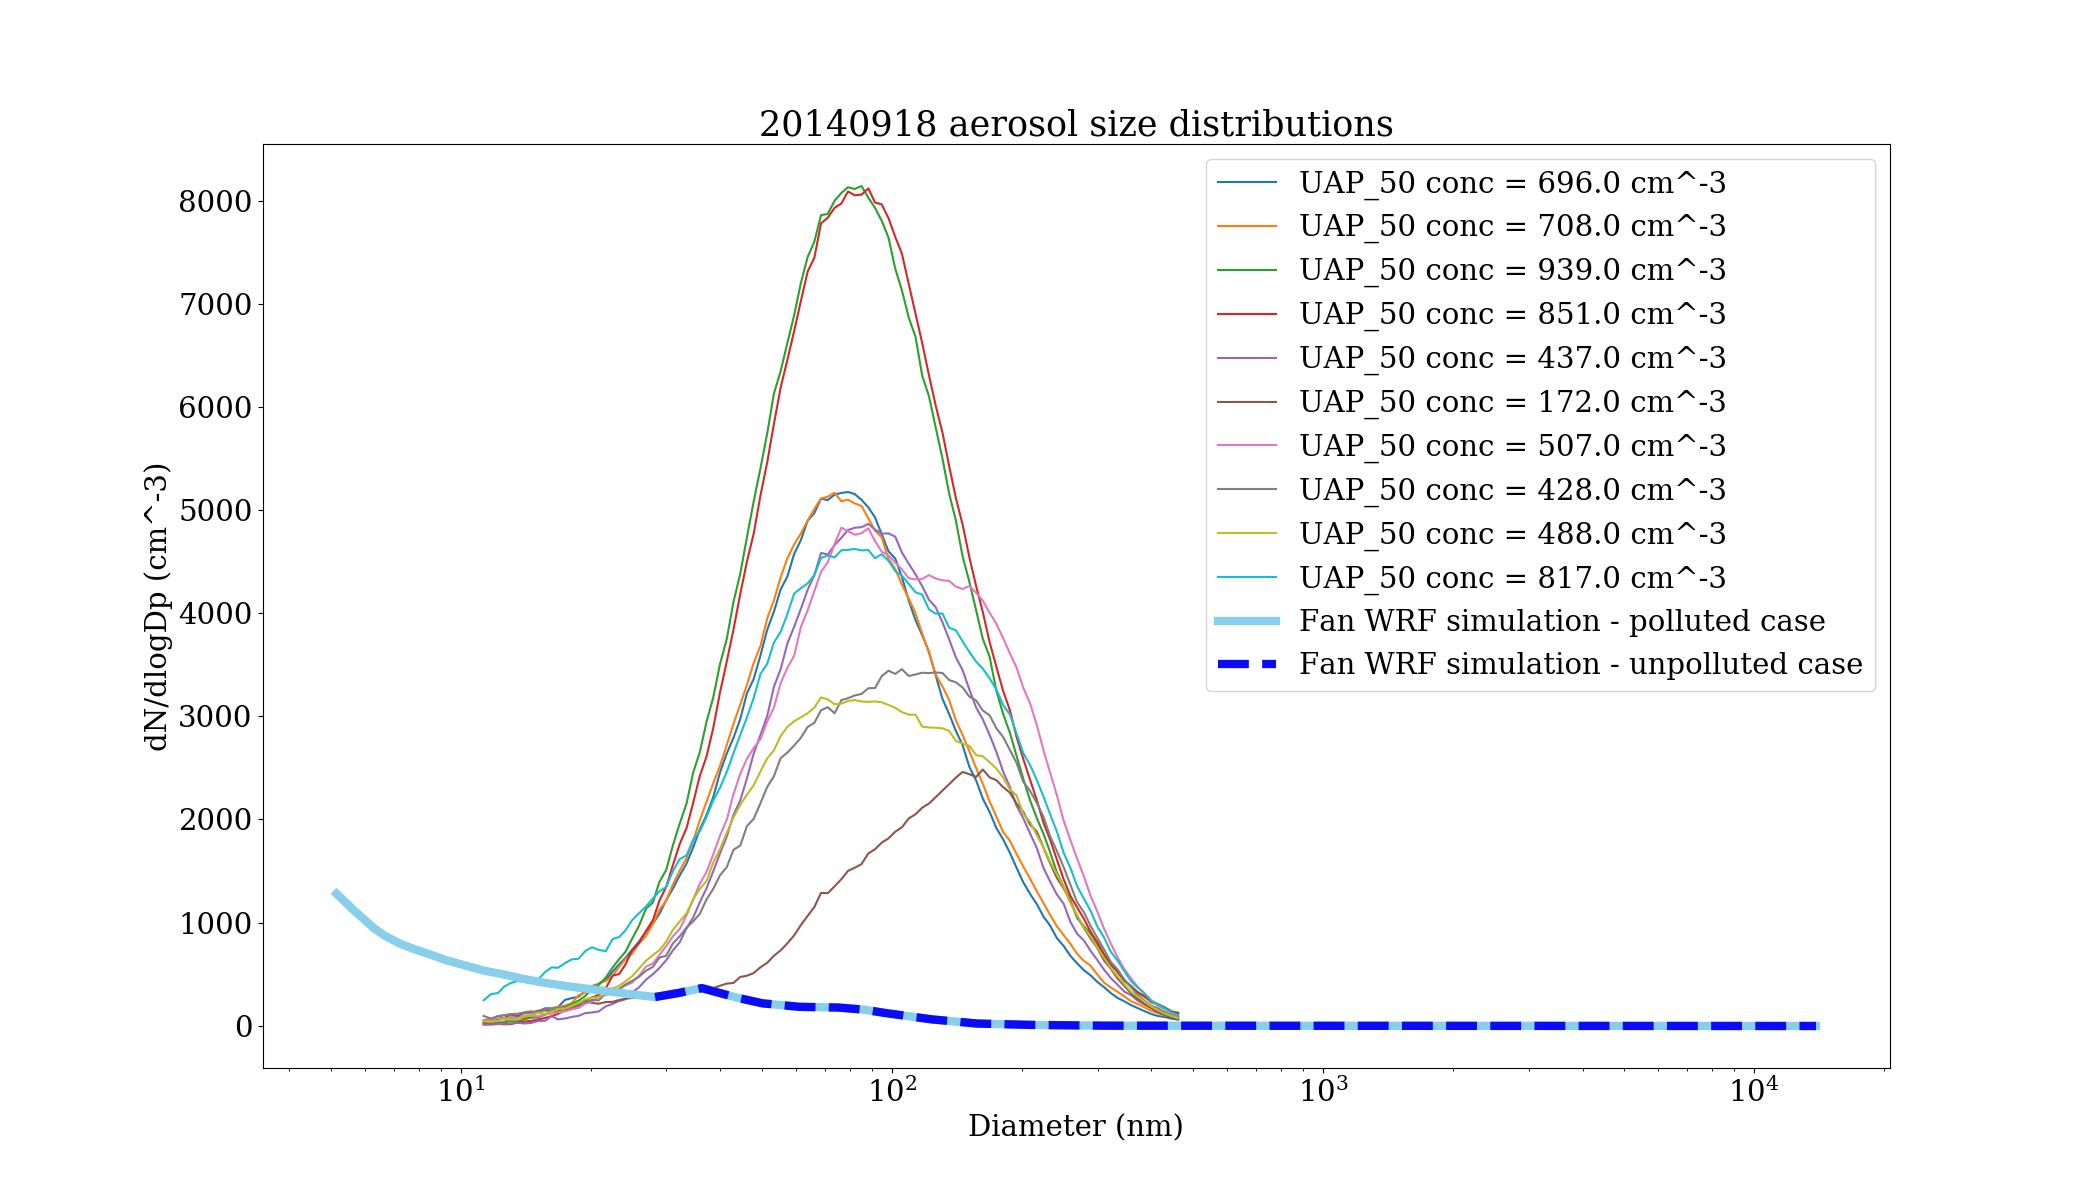
\includegraphics[width=9cm]{goama/v5_aero_size_distb_20140918_figure.png}
    \caption{Aerosol particle size distribution for a representative date; ground-based measurement coinciding with ACRIDICON-CHUVA flight dates, compared to initial distribution in boundary layer for WRF simulation. Curves represent the average over $\approx$2-hour samples. From GoAmazon site, downwind of Manaus metropolitan area.}
    \label{goaasd}
\end{figure}

Even though UAP50 levels in the BL approach the lower bound of what Fan et al used in their simulations (??? pending ATTO measurements from Mira Pohlker), we do not find any supersaturation values in the troposphere exceeding 1\% using the criteria above (Figure \ref{haloqsshist}). The average value of $SS_{QSS}$ measured at all points satisfying the above filtering criteria is 0.23\% (std. dev. 0.15\%). Of those points, we find the average $SS_{QSS}$ for the top tenth percentile of updrafts (as measured by vertical wind velocity) is 0.32\% (std. dev. 0.18\%). [NOTE: Need to do quantitative error analysis on these data]

\clearpage
\newpage

\begin{figure}[ht]
    \centering
    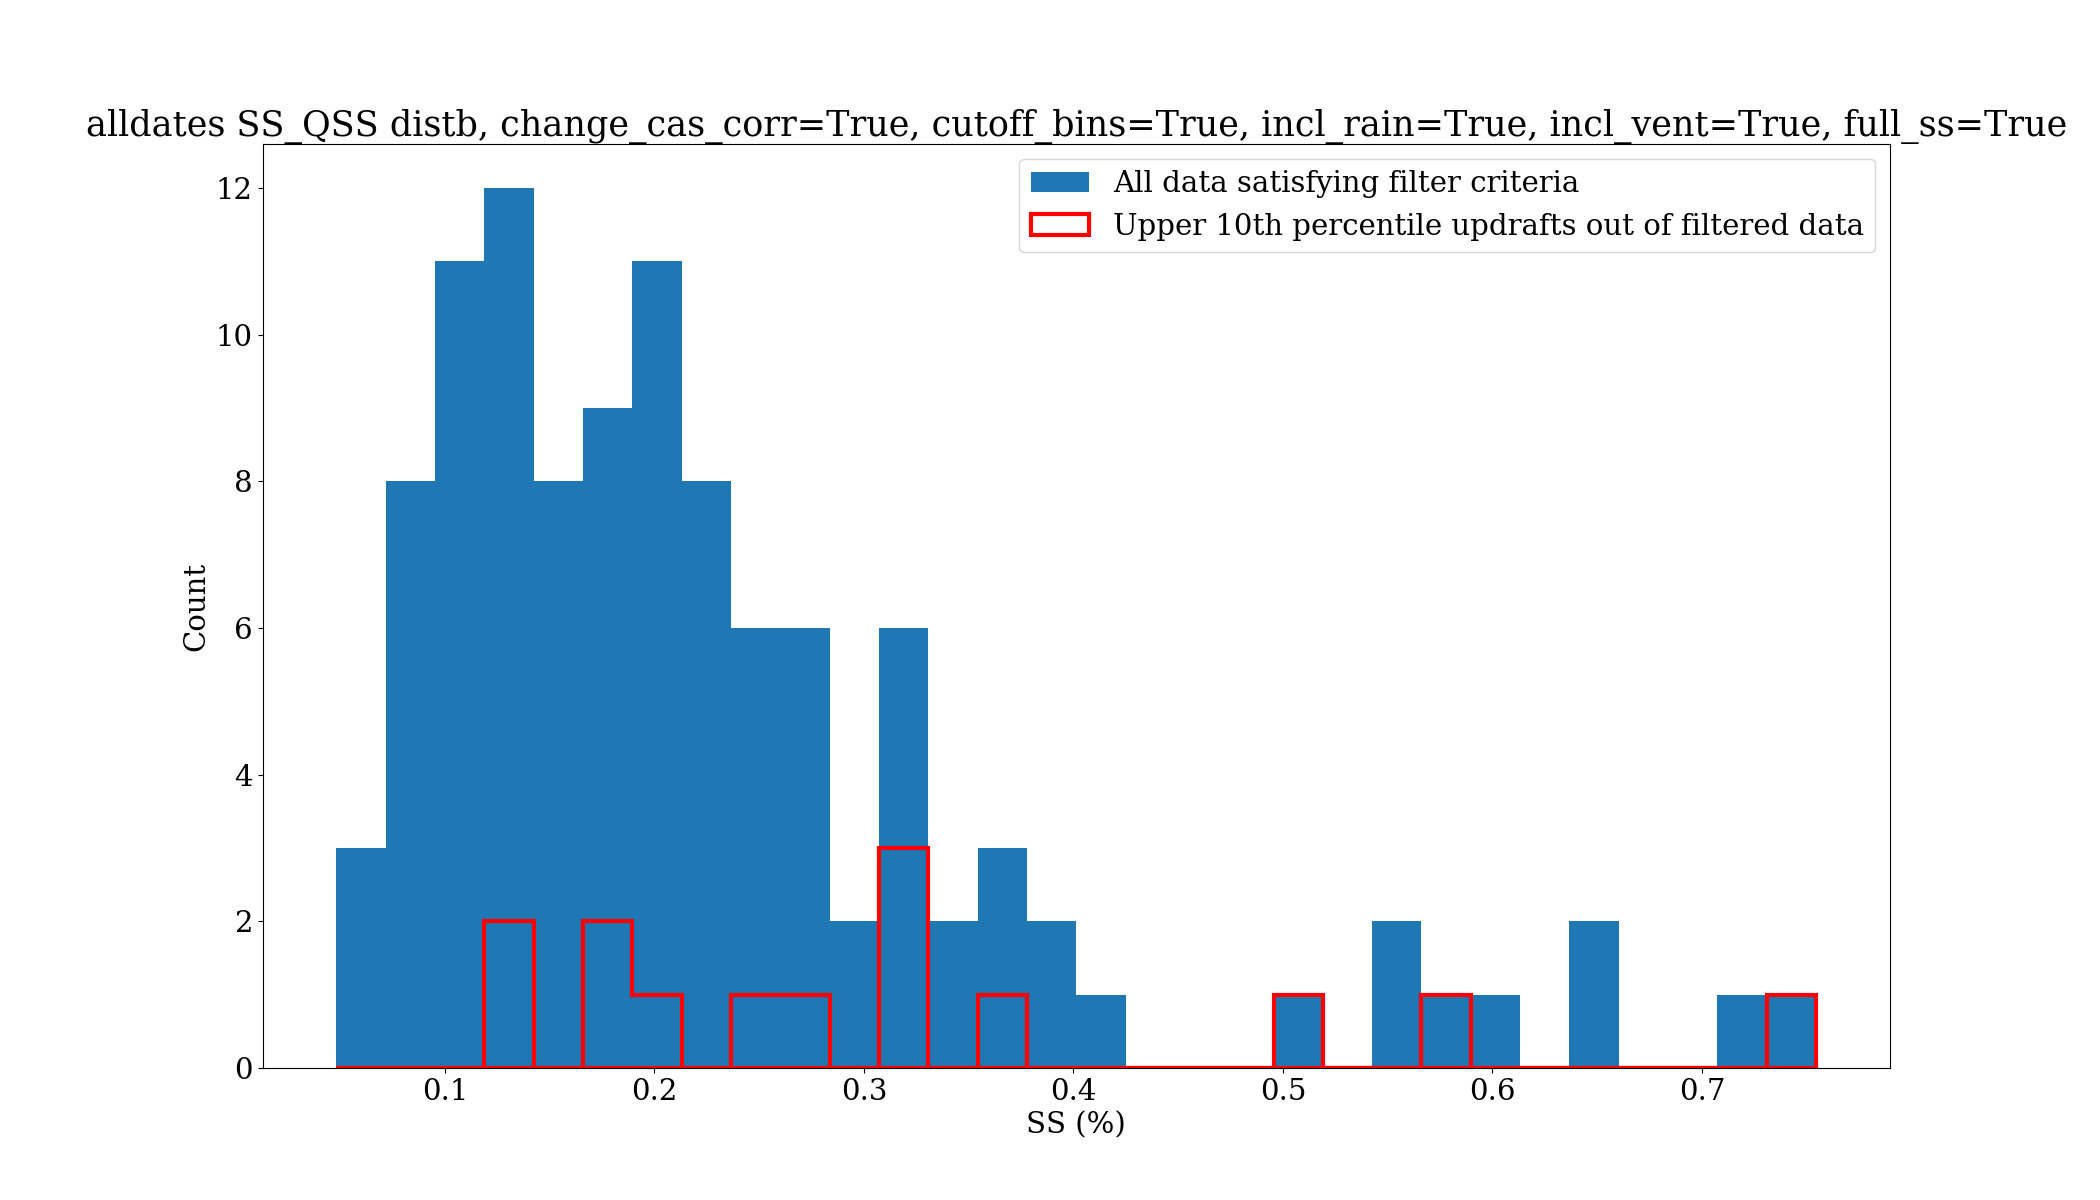
\includegraphics[width=9cm]{revhalo/v24_with_up10perc_ss_qss_hist_cas_alldates_figure.png}
    \caption{Predicted ($SS_{QSS}$) supersaturation distribution from HALO field campaign (all flight dates). Using filtering criteria outlined in the text. Overlying histogram in red is the distribution for points lying in the upper tenth percentile of updrafts (as measured by vertical wind velocity), after Fan 2018.}
    \label{haloqsshist}
\end{figure}

Next we look at data from the CAIPEEX experiment in India. No ground-based aerosol concentration measurements are available (and measurements in the troposphere from instruments on the plane are sketchy...). Supersaturation distribution using the same criteria is shown (for all flight dates combined) in Figure \ref{caipeexqsshist}. We see a relatively small number of supersaturation values exceeding 1\%. The average value of $SS_{QSS}$ measured at all points satisfying the above filtering criteria is 0.49\% (std. dev. 0.64\%). Of those points, we find the average $SS_{QSS}$ for the top tenth percentile of updrafts (as measured by vertical wind velocity) is 0.90\% (std. dev. 0.96\%). [NOTE: Need to do quantitative error analysis on these data]

\begin{figure}[ht]
    \centering
    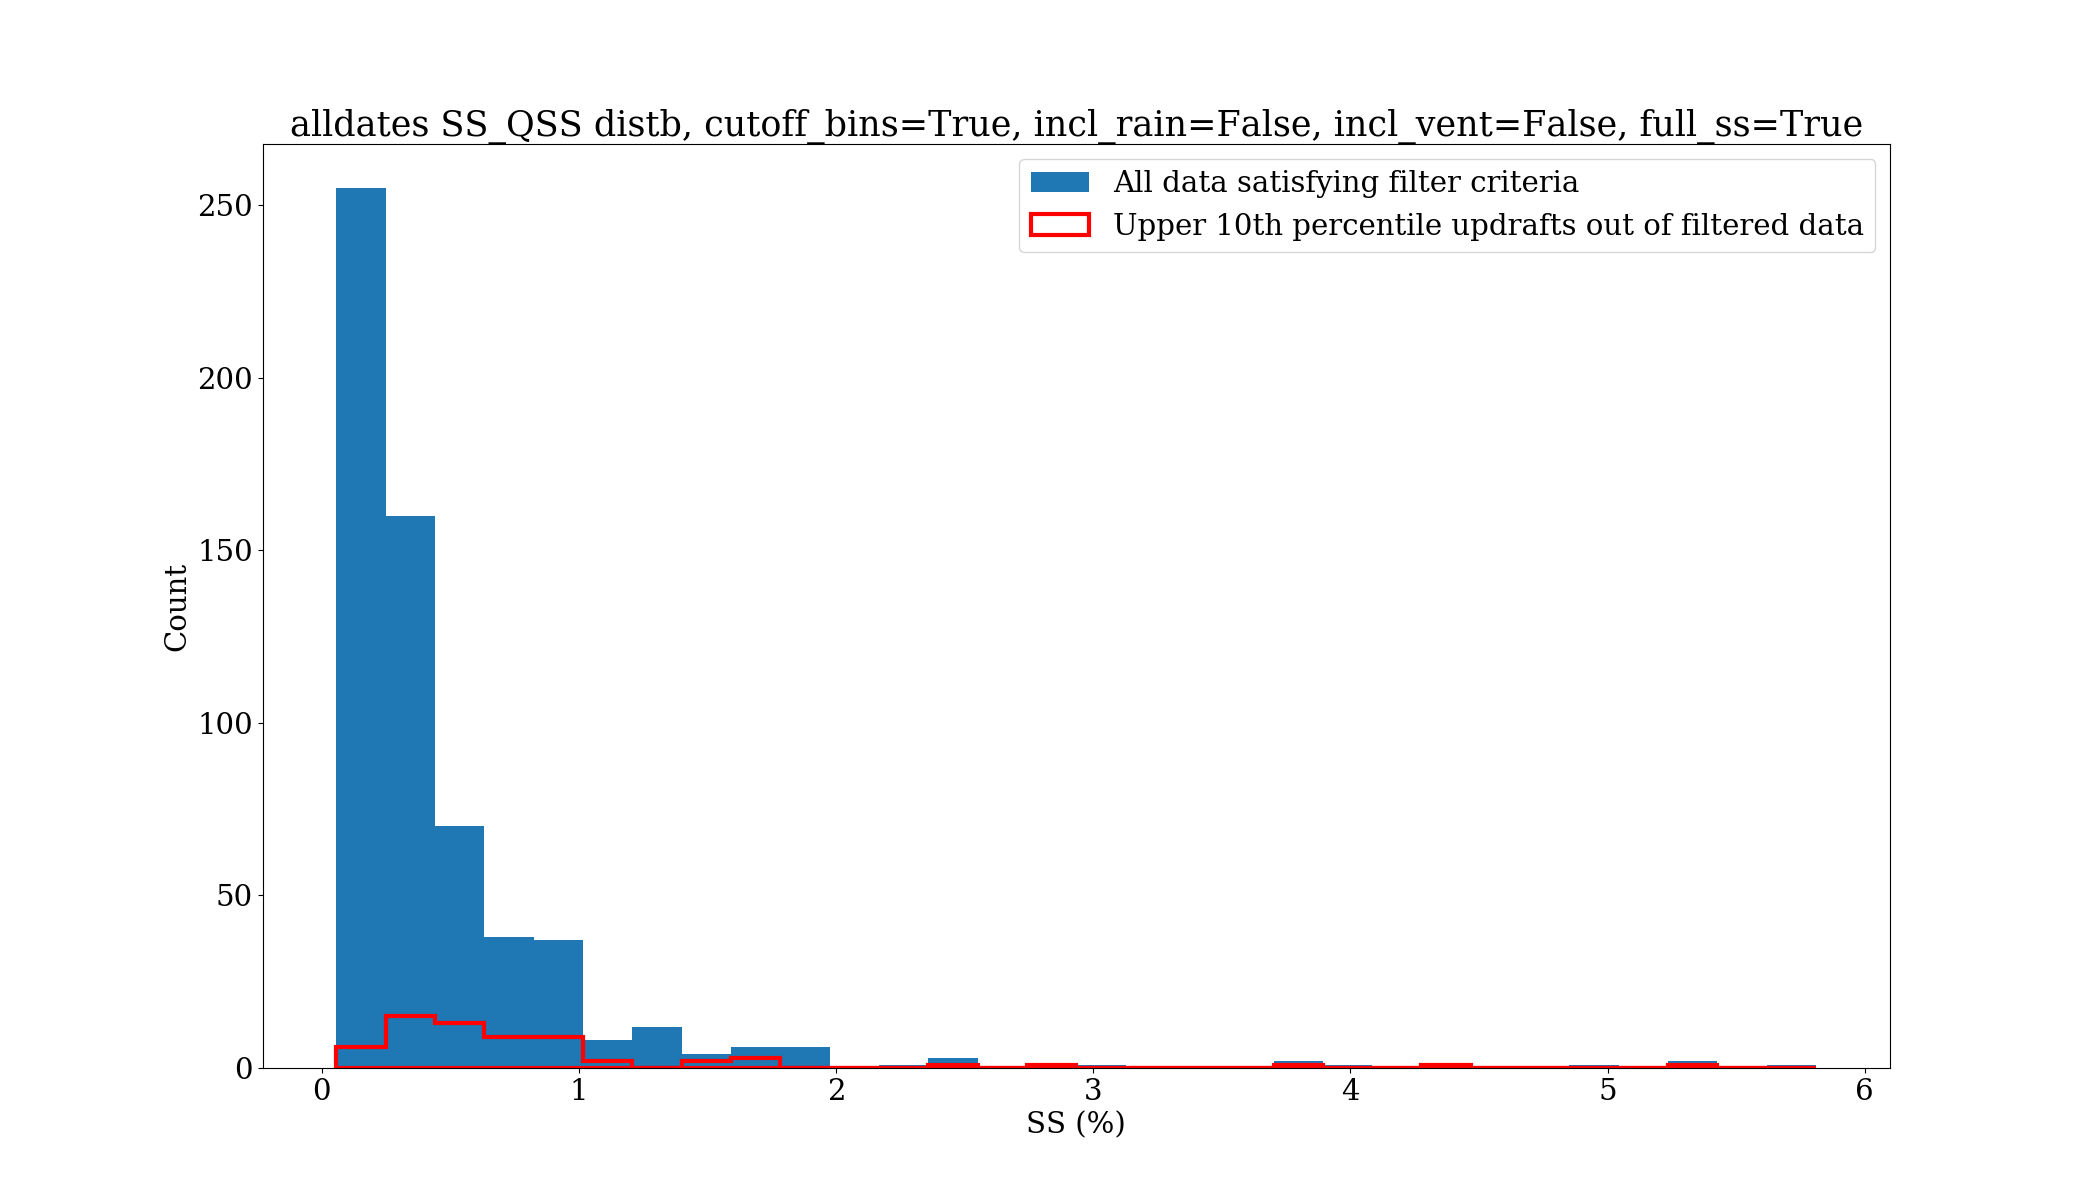
\includegraphics[width=9cm]{revcaipeex/v10_with_up10perc_ss_qss_hist_alldates_figure.png}
    \caption{Predicted ($SS_{QSS}$) supersaturation distribution from CAIPEEX field campaign (all flight dates). Using filtering criteria outlined in the text, but not including rain drops or ventilation corrections due to lack of data. Overlying histogram in red is the distribution for points lying in the upper tenth percentile of updrafts (as measured by vertical wind velocity), after Fan 2018.}
    \label{caipeexqsshist}
\end{figure}

Conclusion: Fan gets a difference in supersaturation (between polluted and clean) of 5\% (11\%) for the warm (deep) cloud phase (averaged over the top tenth percentile of convective updrafts), which supports 100 J/kg (200 J/kg) of invigoration in the polluted case. Here, we find average supersaturations in the top tenth percentile of convective updrafts to be 0.9\% and 0.3\% in CAIPEEX and HALO, respectively, which would support only $\approx$ 1 J/kg invigoration relative to a storm with zero supersaturation [Note this argument is still somewhat contingent on better aerosol data esp. from the ATTO experiment...could just be we are only looking at polluted environments in these field campaigns]. 

One possible counterargument is that the flight campaigns simply didn't fly through strong enough updrafts. However the vertical velocity distributions from the campaigns are quite similar to that from the simulations [can back this up with statistical analysis]. See Figure \ref{combinedwhist}. 

\begin{figure}[ht]
    \centering
    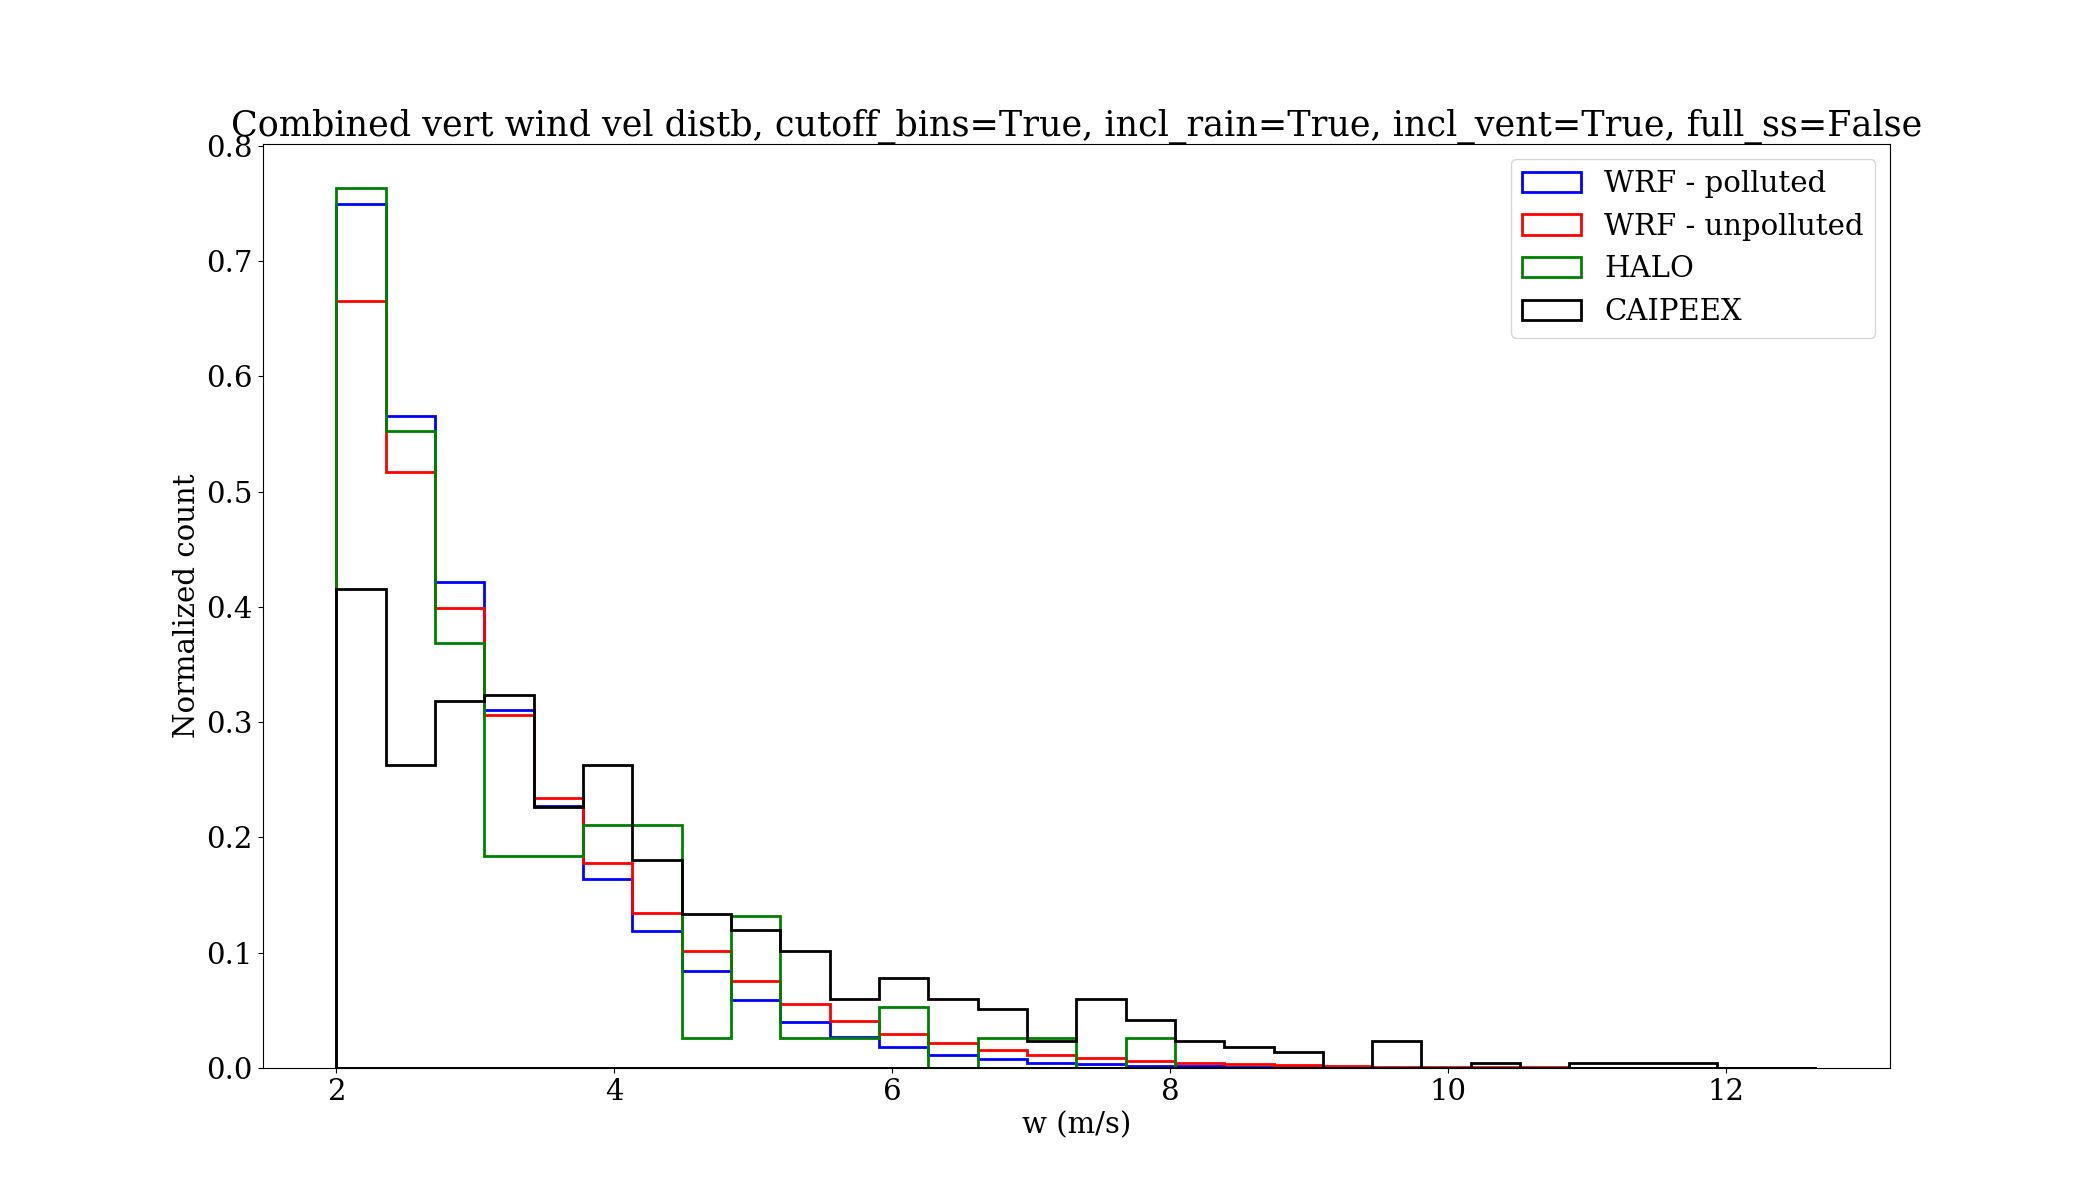
\includegraphics[width=12cm]{revmywrf/v9_combined_w_hist_figure.png}
    \caption{Vertical wind velocity distribution from simulations and field campaigns. Using filtering criteria outlined in the text.}
    \label{combinedwhist}
\end{figure}

\end{document}
